\documentclass[a4paper,14pt,russian]{report}
\usepackage[utf8]{inputenc}
\usepackage[T2A]{fontenc}
\usepackage{extsizes}
\usepackage{amsmath}
\usepackage{listings}
\usepackage{xcolor}
\usepackage{tabularx}
\usepackage{geometry}
\usepackage{titlesec}
\usepackage{graphicx}
\usepackage[font=small,labelfont=bf]{caption}
\usepackage{indentfirst}

\newcommand{\insertInstitute}{
  Институт компьютерных наук и технологий\linebreak
  Высшая школа киберфизических систем и управления
}
\newcommand{\insertTitle}{ОТЧЕТ\par по дисциплине «Инженерная и компьютерная графика»\par \textbf{Построение схемы программы}}
\newcommand{\insertAuthor}{С А. Новиков}
\newcommand{\insertAuthorPosition}{студент гр 13532/1}
\newcommand{\insertVerifier}{А А. Ефремов}
\newcommand{\insertVerifierPosition}{доцент, кф.-м.н}

\newcommand{\sectionbreak}{\clearpage}
\newcommand{\subsectionbreak}{\clearpage}

\graphicspath{ {./images/} }
\renewcommand{\figurename}{Рисунок}
\renewcommand{\tablename}{Таблица}

\sloppy

\linespread{1.3}
\definecolor{lightgray}{gray}{0.95}
\renewcommand{\contentsname}{Содержание}
\renewcommand{\thesection}{\arabic{section}}
\newgeometry{left=3cm,right=2cm,top=2cm,bottom=2cm}
\setlength{\parindent}{1.25cm}
\lstset{
  backgroundcolor=\color{lightgray},
}


\begin{document}

\pagenumbering{gobble}
\begin{center}
  Министерство науки и высшего образования РФ\linebreak
  Санкт-Петербургский политехнический университет\linebreak
  Петра Великого\linebreak
  \insertInstitute\linebreak
\end{center}
\vspace{1.5cm}
\begin{tabularx}{\textwidth}{Xr}
  УДК $\rule{4cm}{0.15mm}$ & УТВЕРЖДАЮ \\
                           & $\rule{5cm}{0.15mm}$ \\
                           & $\rule{5cm}{0.15mm}$ \\
                           & $\rule{5cm}{0.15mm}$ \\
                           & «$\rule{0.8cm}{0.15mm}$» $\rule{2cm}{0.15mm}$ $\rule{1.1cm}{0.15mm}$ г. \\
\end{tabularx}
\vspace{1.5cm}
\begin{center}
  \insertTitle\par
\end{center}
\vspace{1.5cm}
\begin{tabularx}{1\textwidth}{Xll}
  \textbf{Выполнил:}    & & \\
  \insertAuthorPosition & $\rule{3.5cm}{0.15mm}$ & \insertAuthor \\
                        & подпись, дата & \\
  \textbf{Проверил:}      & & \\
  \insertVerifierPosition & $\rule{3.5cm}{0.15mm}$ & \insertVerifier \\
                          & подпись, дата & \\
\end{tabularx}
\vfill
\begin{center}
  Санкт-Петербург $\rule{1.1cm}{0.15mm}$ г.
\end{center}


\newpage
\pagenumbering{arabic}
\setcounter{page}{2}

\section*{Реферат}

\noindent Отчет 22 с., 9 рис., 7 табл., 2источник. \\
БЛОК-СХЕМА, АЛГОРИТМ, ПРОГРАММИРОВАНИЕ \\
Объектом исследования является построение схемы программы. \\
Цель работы — построить блок-схему алгоритма в двух редакторах:
\begin{enumerate}
  \item Dia Diagram Editor
  \item Draw.io
\end{enumerate}

\tableofcontents

\section{Построение схемы в программе Dia Diagram Editor}

\begin{figure}[!htb]
  \centerline{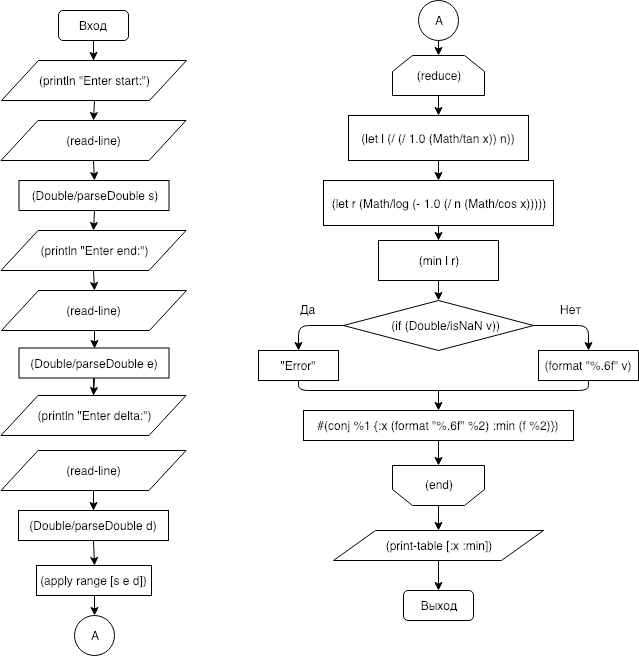
\includegraphics[width=1\textwidth]{dia}}
  \caption{Схема в программе Dia Diagram Editor}
\end{figure}

\section{Построение схемы в программе Draw.io}

\begin{figure}[!htb]
  \centerline{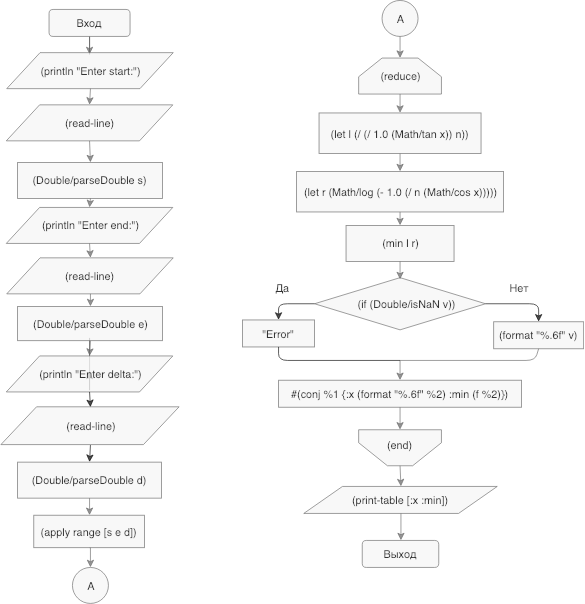
\includegraphics[width=1\textwidth]{draw}}
  \caption{Схема в программе Draw.io}
\end{figure}

\section{Список используемой литературы}

\begin{enumerate}
  \item Инженерная графика // Е.Д. Рябков, Л.И. Димент — Санкт-Петербург, СПбГПУ, 2003.
  \item Инженерная графика (машиностроительное черчение) // — М. ИНФРА-М, 2009.
\end{enumerate}

\end{document}
